\section{Launching the game}
The application starts in the main menu shown in \autoref{fig:main_menu}.
From here a new game can be started, a previous save can be loaded, or a save can be deleted.
The user can also view controls, and exit the game.
To start a game for the first time, the user has to click on the "New Game" button which will show the "New Game Screen".

When the game is running the user can press the \keys{\escwin} key to show the main menu or hide it.
While the game is running the main menu will also show a "Resume" button which will resume the game and hide the menu.

\begin{figure}[H]
    \centering
    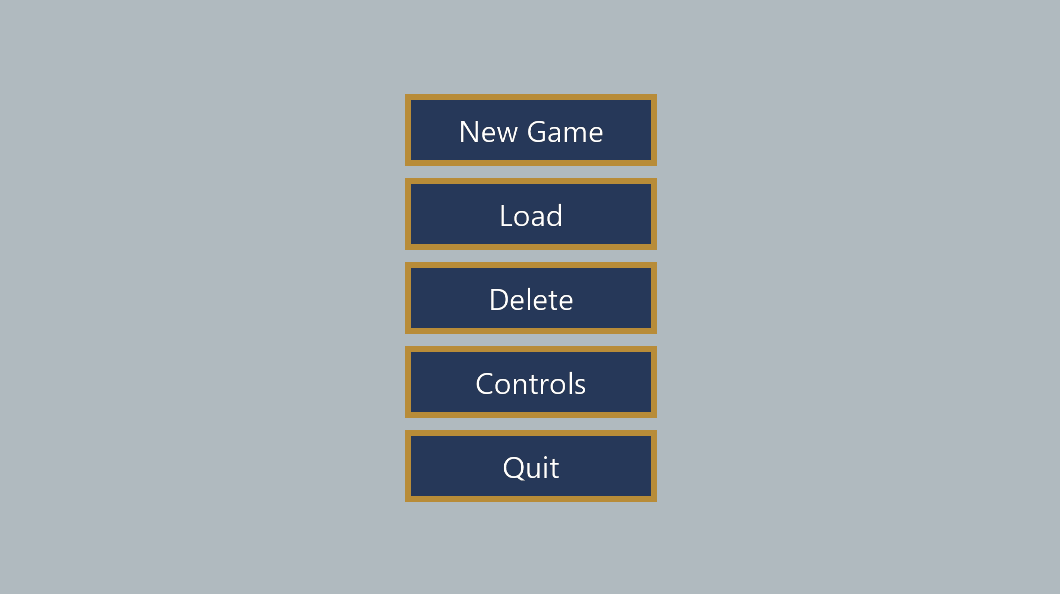
\includegraphics[width=0.8\textwidth]{chapters/user_manual/resources/main-menu.png}
    \caption{Main menu}
    \label{fig:main_menu}
\end{figure}